\documentclass{article} % For LaTeX2e
\usepackage{nips15submit_e,times}
\usepackage{hyperref}
\usepackage{url}
\usepackage{graphicx}
%\documentstyle[nips14submit_09,times,art10]{article} % For LaTeX 2.09


\title{Image Captioning Using LSTM Network}

\author{
Nan Wei \\
UC San Diego\\
\texttt{nwei@ucsd.edu} \\
\And
Renjie Shao \\
UC San Diego \\
\texttt{reshao@ucsd.edu} \\
\And
Hongyi Ling \\
UC San Diego \\
\texttt{holing@ucsd.edu} \\
}

% The \author macro works with any number of authors. There are two commands
% used to separate the names and addresses of multiple authors: \And and \AND.
%
% Using \And between authors leaves it to \LaTeX{} to determine where to break
% the lines. Using \AND forces a linebreak at that point. So, if \LaTeX{}
% puts 3 of 4 authors names on the first line, and the last on the second
% line, try using \AND instead of \And before the third author name.

\newcommand{\fix}{\marginpar{FIX}}
\newcommand{\new}{\marginpar{NEW}}

\nipsfinalcopy % Uncomment for camera-ready version

\begin{document}


\maketitle

\begin{abstract}
    In this article we are dealing with image captioning task on COCO dataset. Here we use a encoder-decoder model while pretrained Resnet50 acts as encoder and LSTM/RNN as decoder. We evaluate our generated captions by perplexity and BLEU score. Our best result reach 9.96 Perplexity, 87.33 BLEU-1 score and 19.02 BLEU-4 score, which verifies our model's performance.

\end{abstract}

\section{Introduction}

    Image captioning is a task to generate captions from images. Normally we want a model to learn from a labeled dataset, i.e. images with captions, can caption new images automatically. To handle this problem, usually we need an encoder to extract features from images and then a decoder to generate texts fro extracted features. In this task we will use pretrained Resnet50 \cite{he2016deep} as our encoder. For decoder, we will use LSTM/RNN to generate texts. The dataset we use is COCO \cite{lin2014microsoft}.


\section{Method}
In this section we will talk about the architecture of our model. The framework of our model is shown as Figure \ref{frame}. We feed our images to ResNet and get an output vector of 2048 dimensions. Then we use a linear layer to map our feature vector to 300 dimensions, which is the embedding dimensions. This 300 dimensions vector will act as input to feed into our LSTM/RNN network. Then we use teaching force to train our decoder, for each time step, we use current label word as next time input to our decoder, i.e. $x(t+1)=target(t)$. Note that each word first go through the embedding layer, which will transfer them into 300 dimensions vector.

\begin{figure}[htb!]
    \centering
     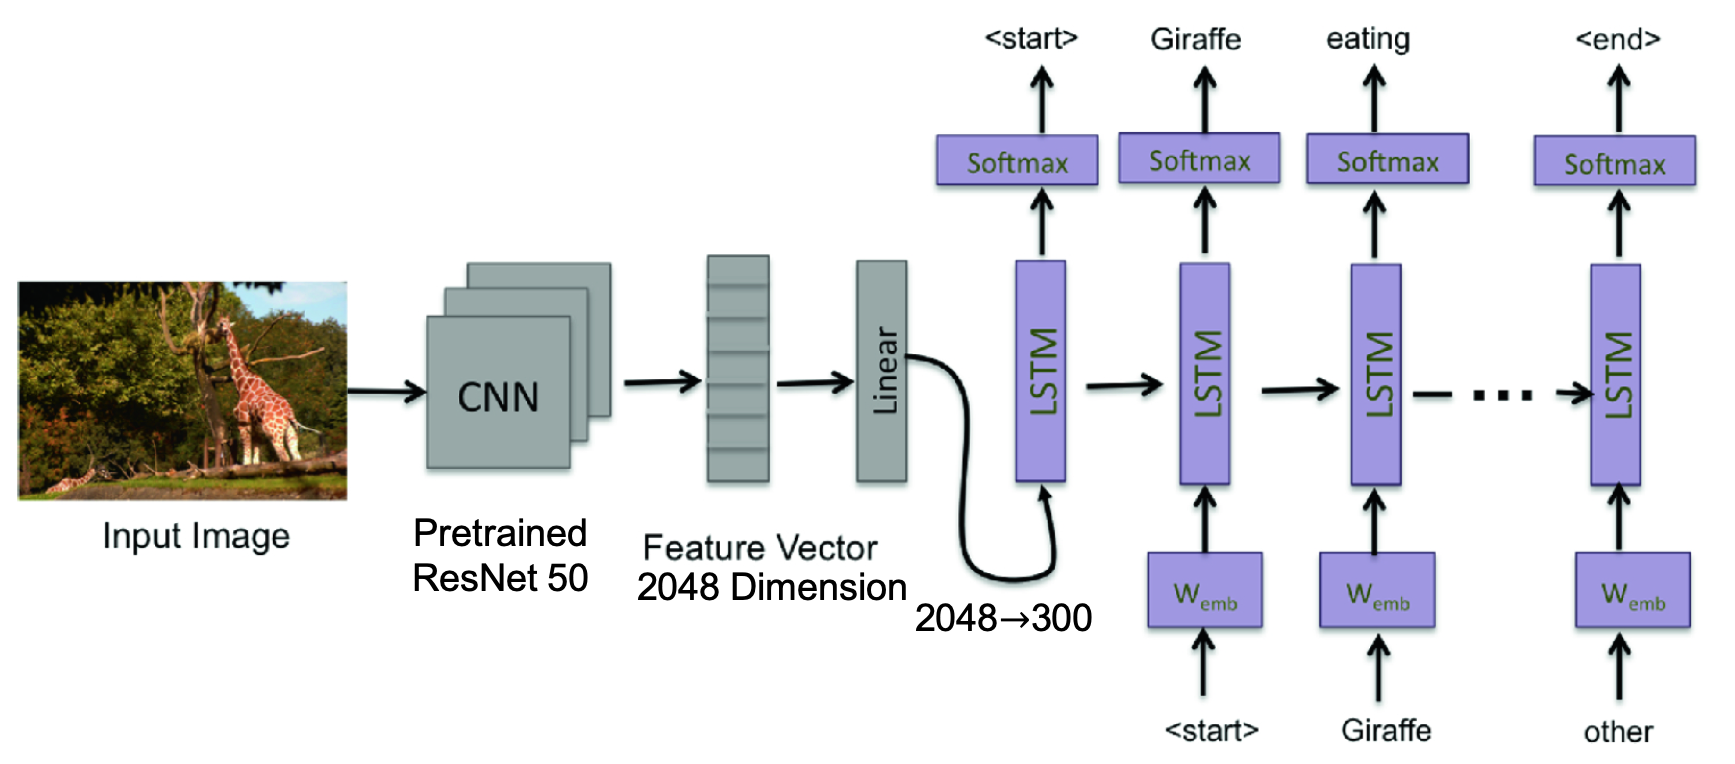
\includegraphics[width=0.8\textwidth]{frame}
    \caption{Model Framework \cite{10.1007/978-3-030-04780-1_23}}
    \label{frame}
\end{figure}

In this task we will try LSTM and RNN as our decoder and compare the performances between them. Also, we will also use pretrained word embedding to see if this may improve our performance. The word embedding we use here is GloVe.6B with 300 embedding dimensions \cite{pennington2014glove}. For baseline LSTM and RNN model, we use random initialized word embedding and fine tuning during the training process. Pretrained word embedding are widely used in NLP tasks. The advantages to use pretrained word embeddings is that it usually trained in a  vary larger dataset with longer training process, which enhances the expressive capacity of each word vector. For example, the GloVe.6B we use are trained on 6 billion tokens. Hopefully, we want to see improvement after using this word embedding.

The detailed parameters and hyper-parameters for each models are listed in Table \ref{para}. Since LSTM has more parameters than RNN at each unit, here we use 2 layers RNN to make a compromise.

\begin{table}[!htb]
    \centering
    \begin{tabular}{l|l|l|l|l|l|l|l}
        \hline
        Model & Encoder & Embed Dim & Hidden Dim & Layer &  Optimizer & LR & $L_2$ Penalty \\
        \hline
        LSTM(baseline) & Resnet50 &  300& 512 & 1 & Adam & 0.001 & $10^{-5}$ \\
        \hline
        RNN & Resnet50 & 300 & 512 & 2 & Adam & 0.001 & $10^{-5}$ \\
	    \hline
		LSTM+GloVe& Resnet50 & 300 & 512 & 1 & Adam & 0.001 & $10^{-5}$ \\
	    \hline
    \end{tabular}
    \caption{Hyper-parameters for different models}
    \label{para}
\end{table}



\section{Experiments}
In this section, we will show the training process for each models and compare the performances in different indices such as perplexity, BLEU score.

\subsection{Training curve}

Firstly let us see the training curve for baseline LSTM and RNN, which is shown as Figure \ref{loss_lstm_no}, \ref{RNNloss}.

\begin{figure}[htb!]
    \begin{minipage}[t]{0.48\textwidth}
        \centering
        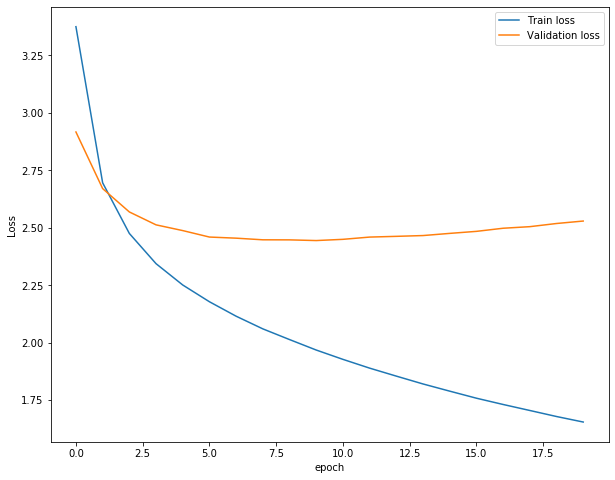
\includegraphics[width=0.9\textwidth]{lstm_no_pretrain_loss.png}
       \caption{Training curve of LSTM}
       \label{loss_lstm_no}
    \end{minipage}
    \begin{minipage}[t]{0.48\textwidth}
        \centering
        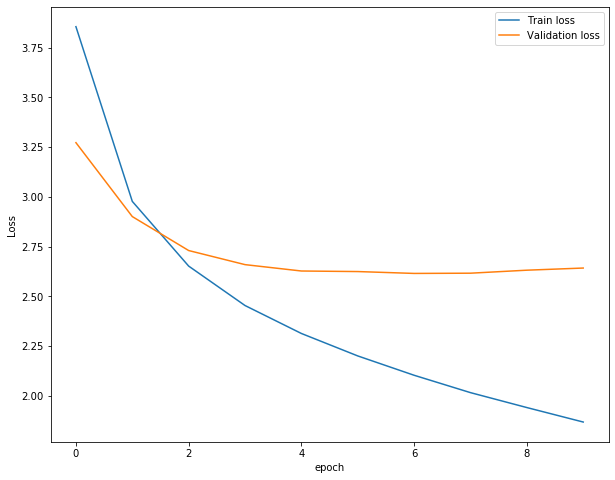
\includegraphics[width=0.9\textwidth]{RNNloss}
        \caption{Training curve of vanilla RNN}
        \label{RNNloss}
    \end{minipage}
\end{figure}

As we can see, LSTM converges at 10 epochs while RNN at 6. Though our RNN has two layers and LSTM only has one, it still takes more time for LSTM to converge. However, the validation loss of LSTM is slightly better than RNN. Firstly, a LSTM cell unit has more parameters than RNN, so it is reasonable LSTM need more time to train. Also since LSTM has stronger ability to catch long-term dependency, it performs better than RNN in loss. 

\subsection{Pretrained Word Embedding}

Here we will see the learning curve of LSTM with pretrained GloVe word embeddings. The learning curve is shown as Figure \ref{LSTM_pre_loss}. As we can see, LSTM with pretrained word embedding converges faster than baseline LSTM. This is because by using pretrained word embeddings, we do not need much time to train our embedding layer. The validation loss of both model is near, which implies that by several epochs our baseline model can learn a good embedding for words. 


\begin{figure}[htb!]
    \centering
     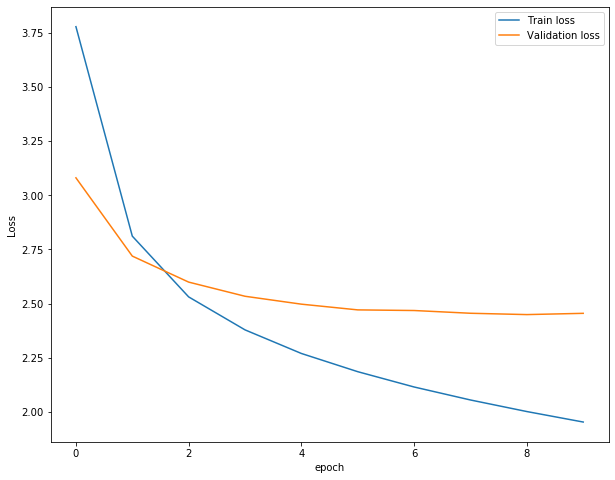
\includegraphics[width=0.7\textwidth]{LSTM_pretrainedloss}
    \caption{Training and validation loss of LSTM with pretrained embedding}
    \label{LSTM_pre_loss}
\end{figure}

\subsection{Perplexity and BLEU}

Now we move on to the evaluation of our models. In generation tasks, perplexity is a widely used index to evaluate the generated texts. Its definition is
\begin{equation}
    ppl = \exp (-\sum_x p(x)\log p(x)).
\end{equation}
Perplexity is a measurement of how well a probability distribution or probability model predicts a sample. The smaller perplexity we have, the better prediction it will give. So perplexity gives a probability evaluation of our model. BLEU (bilingual evaluation understudy) \cite{papineni2002bleu} is another way to measure our model. It use $n$-gram model to compute the correlation of machine output and labels. Here we use BLEU-1 and BLEU-4 scores to evaluate our models.

The results of different model is shown as Table \ref{bleu}. As we can see, LSTM models has better performance than RNN in all indices. It proves that, with the capacity of catch long-term dependency, LSTM is more powerful than RNN. Also note that LSTM-GloVe is slightly better than baseline model. It shows that with efficient training, our baseline can learning a good word embedding. And also note that in BLEU-4, LSTM-GloVe has better performance. So pretrained word embeddings still show improvement. It is a good idea to try pretrained word embedding when doing NLP tasks.

\begin{table}[htb!]
    \centering
    \begin{tabular}{l|c|c|c|c}
        \hline
        Model & Loss & Perplexity & BLEU-1 & BLEU-4 \\
        \hline
        LSTM & 2.29 & 9.96 & 87.33 & 17.04 \\
        \hline
        LSTM+GloVe& 2.30 & 9.97 &87.31&19.02\\\hline
        RNN & 2.46 & 11.68 & 87.04 & 17.22 \\
	    \hline
    \end{tabular}
    \caption{Performance for different models}
    \label{bleu}
\end{table}

\subsection{Stochastic Approach}

When choosing the generated word, formerly we always choose the one with maximum probability. By this way we always generates texts most likely to training set probability distribution. However, it also has disadvantages. The key problem of this method is that it will cause our generated corpus losing variety. To solve this problem, here we will try a stochastic approach, i.e., to sample words with weights as
\begin{equation}
    y^{j}=\exp \left(o^{j} / \tau\right) / \sum_{n} \exp \left(o^{n} / \tau\right),
\end{equation}
where $o^j$ is the output of last layer, $n$ is the size of vocabulary and $\tau$ is the hyper-parameter `temperature'.


Here we try several different temperature and calculate the BLEU score on our baseline model. The result is shown in Table \ref{baseline_table}. We can see that when $\tau = 0.1$ the model performs best. When temperature is very small, stochastic approach is close to deterministic approach. With $\tau$ grows, the BLEU scores decrease. And also, all of them are worse than deterministic approach. This is because deterministic approach always make decision that lead generated texts as close to references as possible, so when evaluated on BLEU scores, it performs better. However, stochastic approach can still give variety to our generated corpus, which is useful in some real tasks.


\begin{table}[htb!]
    \centering
    \begin{tabular}{l|l|l|l|l|l|l}
    \hline
    Temperature & 0.1   & 0.2   & 0.7   & 1     & 1.5   & 2     \\\hline
    BLEU-1      & 87.29 & 87.22 & 87.05 & 85.89 & 72.19 & 55.73 \\\hline
    BLEU-4      & 17.3  & 17.13 & 15.41 & 13.16 & 5.66  & 3.48 \\\hline
    \end{tabular}
    \caption{BLEU scores for baseline model with stochastic approach}
    \label{baseline_table}  
\end{table}

\section{Conclusion}

In this article we test three models: LSTM, LSTM+GloVe and RNN, and two different sample approach: deterministic and stochastic. The experiments shows that all models are powerful with LSTM+GloVe has the best performance. Our work shows that CNN encoder plus RNN/LSTM decoder is a useful framework to do image captioning.

\section{Individual Contribution}

\subsection*{Nan Wei}
I implement BLEU evaluation, run and test RNN model. I also write related parts in report.

\subsection*{Renjie Shao}
I implement data loader, model framework and help debug. I also write the report.
\subsection*{Hongyi Ling}
I implement the generation part of our model and do experiments on baseline model.  In addition, I write parts of the report.

\bibliographystyle{unsrt}
\bibliography{references}


\end{document}
